\documentclass[border=10pt,tikz]{standalone}
\usepackage{tikz}
\usetikzlibrary{calc,angles,quotes}
\begin{document}
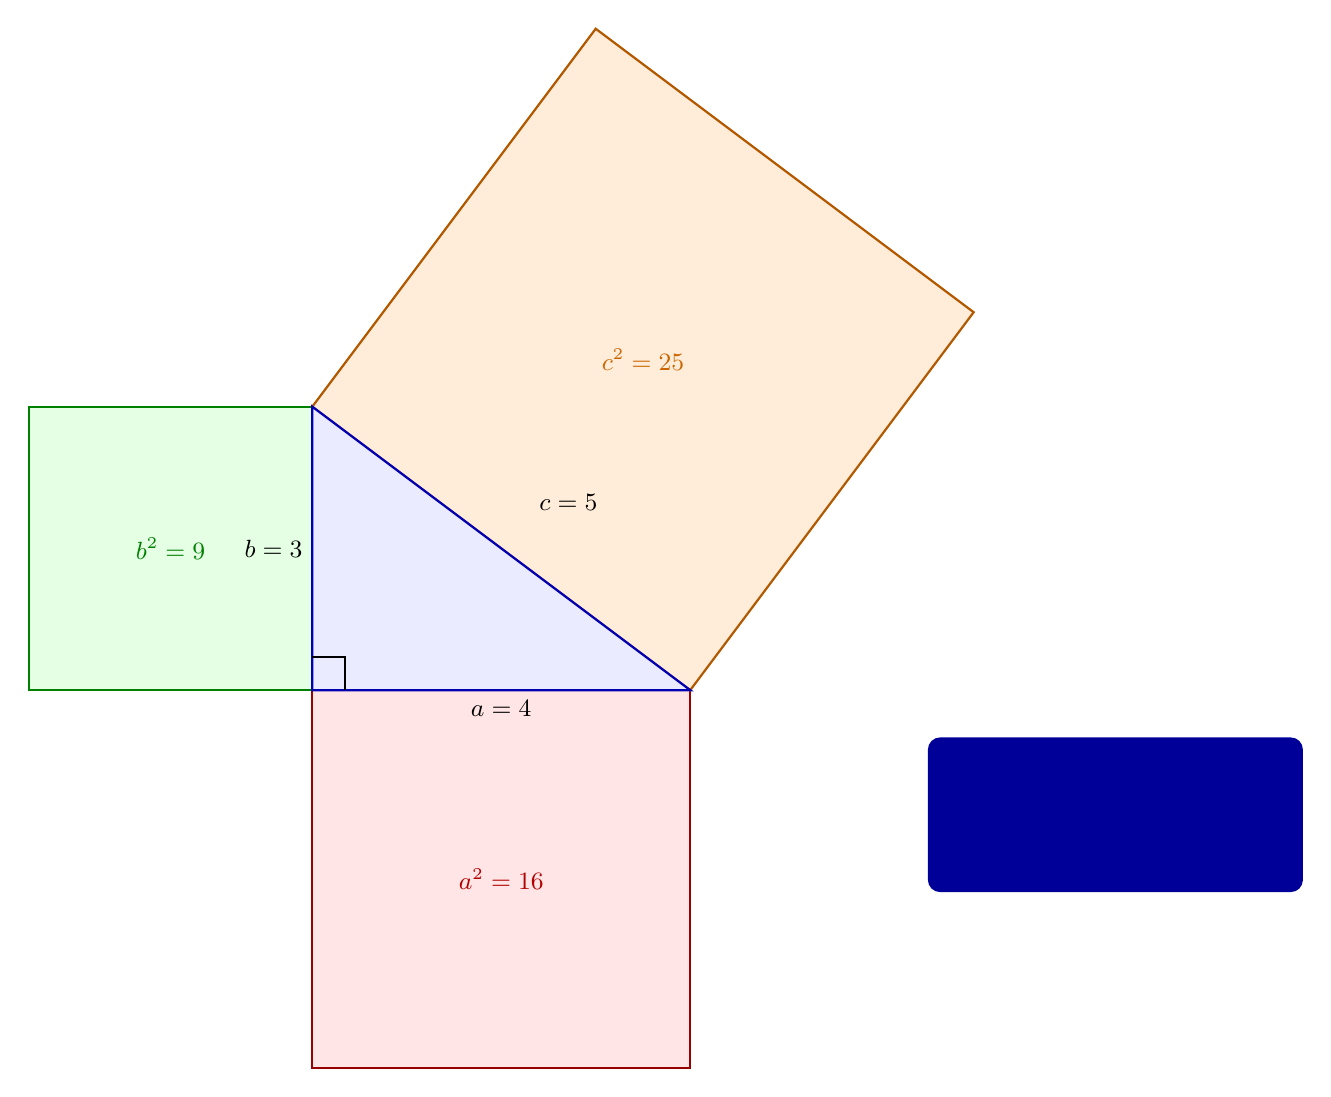
\begin{tikzpicture}[scale=1.2, font=\sffamily\small]

  % Koordinat segitiga siku-siku
  % a = 4 (alas), b = 3 (tegak), c = 5 (sisi miring)
  \coordinate (A) at (0,0);   % sudut siku
  \coordinate (B) at (4,0);   % sisi alas (a = 4)
  \coordinate (C) at (0,3);   % sisi tegak (b = 3)

  % --- Kuadrat di sisi a (bawah), panjang 4 → persegi 4×4 ---
  \fill[red!10]  (0,0) -- (4,0) -- (4,-4) -- (0,-4) -- cycle;
  \draw[thick, red!60!black] (0,0) -- (4,0) -- (4,-4) -- (0,-4) -- cycle;
  \node[red!70!black] at (2,-2) {$a^2 = 16$};

  % --- Kuadrat di sisi b (kiri), panjang 3 → persegi 3×3 ---
  \fill[green!10] (0,0) -- (0,3) -- (-3,3) -- (-3,0) -- cycle;
  \draw[thick, green!50!black] (0,0) -- (0,3) -- (-3,3) -- (-3,0) -- cycle;
  \node[green!50!black] at (-1.5,1.5) {$b^2 = 9$};

  % --- Kuadrat di sisi miring c (hipotenusa), panjang 5 → persegi 5×5 ---
  % Hipotenusa: B(4,0) → C(0,3), vektor arah = (-4,3)
  % Rotasi 90° searah jarum jam (keluar segitiga): (3,4)
  % B + (3,4) = (7,4),  C + (3,4) = (3,7)
  \fill[orange!15] (4,0) -- (7,4) -- (3,7) -- (0,3) -- cycle;
  \draw[thick, orange!70!black] (4,0) -- (7,4) -- (3,7) -- (0,3) -- cycle;
  \node[orange!80!black] at (3.5,3.5) {$c^2 = 25$};

  % Segitiga utama (di atas, supaya tidak tertutup square)
  \fill[blue!8] (A) -- (B) -- (C) -- cycle;
  \draw[thick, blue!70!black] (A) -- (B) -- (C) -- cycle;

  % Tanda sudut siku
  \draw[thick] (0.35,0) -- (0.35,0.35) -- (0,0.35);

  % Label sisi
  \node[below] at (2,0) {$a = 4$};
  \node[left]  at (0,1.5) {$b = 3$};
  \node[above right] at (2.3,1.8) {$c = 5$};

  % Rumus
  \node[draw, rounded corners, fill=blue!5, thick, blue!60!black,
        text width=4.5cm, align=center, anchor=north]
    at (8.5,-0.5)
    {\textbf{Teorema Pythagoras}\\[4pt]
     $a^2 + b^2 = c^2$\\[2pt]
     $16 + 9 = 25$\\[2pt]
     $\sqrt{25} = 5$};

\end{tikzpicture}
\end{document}
